% Implementation

\begin{slide}{Implementation}
  (1) \texttt{connect()} $\longleftrightarrow$ \texttt{accept()}
  \vspace{0.8cm}

  \onslide<2->{
  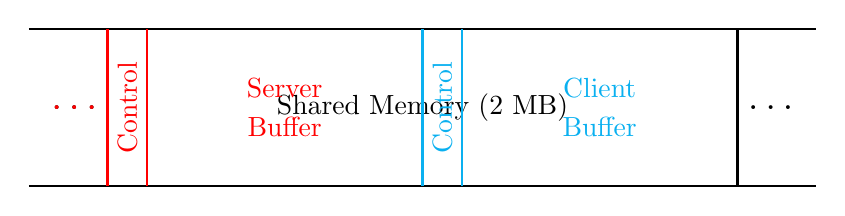
\begin{tikzpicture}

    % Upper/lower border
    \draw [thick] (0, 2) -- ++(10, 0);
    \draw [thick] (0, 0) -- ++(10, 0);

    % Label
    \onslide<2>{
      \draw (5, 1) node {Shared Memory (2 MB)};
      \draw [thick] (1, 0) -- ++(0, 2) node [midway, left] {\black\Large $\dots$};
    }

    % Other memory
    \draw [thick] (9, 0) -- ++(0, 2)
          node [midway, right] {\black\Large $\dots$};

    % Buffer
    \onslide<3>{
      % Control data
      \draw [Red, thick]
            (1, 0) -- ++(0, 2) node [midway, left] {\black\Large $\dots$};
      \draw [Red, thick] (1.5, 0) -- ++(0, 2);
      \draw (1.25, 1) node [Red, rotate=90] {Control};

      \draw [ProcessBlue, thick] (5, 0) -- ++(0, 2);
      \draw [ProcessBlue, thick] (5.5, 0) -- ++(0, 2);
      \draw (5.25, 1) node [ProcessBlue, rotate=90] {Control};

      % Buffer memory
      \foreach \i in {0.5, 1, 2.5, 3} {
        % \draw [Red] ({1.5+\i}, 0) -- ++(0, 2);
        % \draw [ProcessBlue] ({5.5+\i}, 0) -- ++(0, 2);
      }

      % Labels
      \draw [Red] (3.25, 1.25) node {Server};
      \draw [Red] (3.25, 0.75) node {Buffer};

      \draw [ProcessBlue] (7.25, 1.25) node {Client};
      \draw [ProcessBlue] (7.25, 0.75) node {Buffer};

    }
  \end{tikzpicture}
  }
\end{slide}

\begin{slide}{Implementation}
  (2) Client \texttt{write(500 KB)}
  \vspace{0.8cm}

  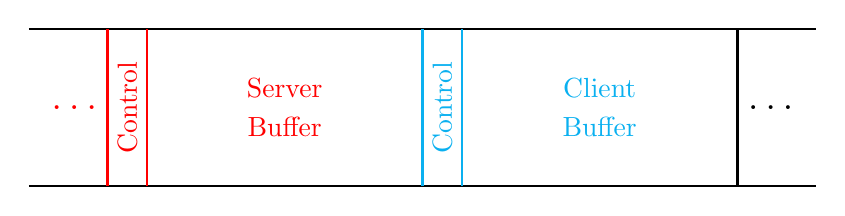
\begin{tikzpicture}

    % Upper/lower border
    \draw [thick] (0, 2) -- ++(10, 0);
    \draw [thick] (0, 0) -- ++(10, 0);

    % Other memory
    \draw [Red, thick] (1, 0) -- ++(0, 2) node [midway, left] {\black\Large $\dots$};
    \draw [thick] (9, 0) -- ++(0, 2)
          node [midway, right] {\black\Large $\dots$};

    % Buffer
    % Control data
    \draw [Red, thick] (1.5, 0) -- ++(0, 2);
    \draw (1.25, 1) node [Red, rotate=90] {Control};

    \draw [ProcessBlue, thick] (5, 0) -- ++(0, 2);
    \draw [ProcessBlue, thick] (5.5, 0) -- ++(0, 2);
    \draw (5.25, 1) node [ProcessBlue, rotate=90] {Control};

    % Buffer memory
    \foreach \i in {0.5, 1, 2.5, 3} {
      % \draw [Red] ({1.5+\i}, 0) -- ++(0, 2);
      % \draw [ProcessBlue] ({5.5+\i}, 0) -- ++(0, 2);
    }

    % Labels
    \draw [Red] (3.25, 1.25) node {Server};
    \draw [Red] (3.25, 0.75) node {Buffer};

    \draw [ProcessBlue] (7.25, 1.25) node {Client};
    \draw [ProcessBlue] (7.25, 0.75) node {Buffer};
  \end{tikzpicture}
\end{slide}

\begin{frame}[fragile]{Implementation}
  \centering
  (2) Client \texttt{write(500 KB)}
  \vspace{0.8cm}

  \begin{lstlisting}
      int write(int fd, void* buffer, int length) {
        if (using_our_library(fd)) {
          connection = lookup(fd);
          return buffer_write(connection, buffer, length);
        } else {
          return real_write(fd, buffer, length);
        }
      }
  \end{lstlisting}
\end{frame}


\begin{slide}{Implementation}
  (2) Client \texttt{write(500 KB)}
  \vspace{0.8cm}

  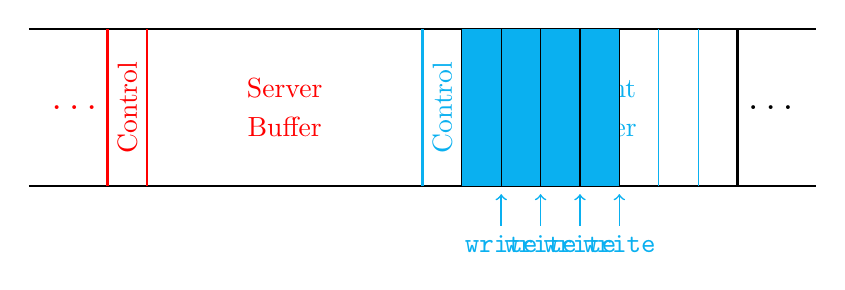
\begin{tikzpicture}

    % Upper/lower border
    \draw [thick] (0, 2) -- ++(10, 0);
    \draw [thick] (0, 0) -- ++(10, 0);

    % Other memory
    \draw [Red, thick] (1, 0) -- ++(0, 2) node [midway, left] {\black\Large $\dots$};
    \draw [thick] (9, 0) -- ++(0, 2)
          node [midway, right] {\black\Large $\dots$};

    % Control data
    \draw [Red, thick] (1.5, 0) -- ++(0, 2);
    \draw (1.25, 1) node [Red, rotate=90] {Control};

    \draw [ProcessBlue, thick] (5, 0) -- ++(0, 2);
    \draw [ProcessBlue, thick] (5.5, 0) -- ++(0, 2);
    \draw (5.25, 1) node [ProcessBlue, rotate=90] {Control};

    % Labels
    \draw [Red] (3.25, 1.25) node {Server};
    \draw [Red] (3.25, 0.75) node {Buffer};

    \onslide<1>{
      \draw [ProcessBlue] (7.25, 1.25) node {Client};
      \draw [ProcessBlue] (7.25, 0.75) node {Buffer};
    }

    \onslide<2->{
      % Client Buffer Memory
      \foreach \i in {0.5, 1, ..., 3} {
        \draw [ProcessBlue] ({5.5+\i}, 0) -- ++(0, 2);
      }
    }

    \foreach \i in {3, ..., 6} {
      \onslide<\i>{
        \draw [->, semithick, ProcessBlue]
              ({6+(\i-3)/2}, -0.5) node [below] {\texttt{write}}
         -- ++(0, 0.4);
        \draw (5.5, 0) -- ++(0, 2);
      }
      \onslide<\i->{
        \draw [fill=ProcessBlue]
              ({5.5+(\i-3)/2}, 0) rectangle ++(0.5, 2);
      }
    }
  \end{tikzpicture}
\end{slide}

\begin{slide}{Implementation}
  (2) Server \texttt{read(250 KB)}
  \vspace{0.8cm}

  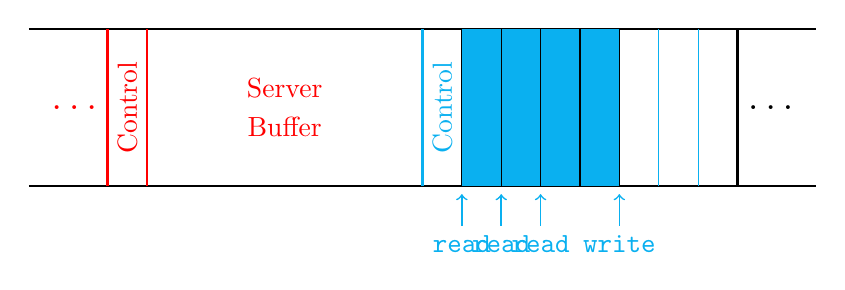
\begin{tikzpicture}

    % Upper/lower border
    \draw [thick] (0, 2) -- ++(10, 0);
    \draw [thick] (0, 0) -- ++(10, 0);

    % Other memory
    \draw [Red, thick] (1, 0) -- ++(0, 2) node [midway, left] {\black\Large $\dots$};
    \draw [thick] (9, 0) -- ++(0, 2)
          node [midway, right] {\black\Large $\dots$};

    % Control data
    \draw [Red, thick] (1.5, 0) -- ++(0, 2);
    \draw (1.25, 1) node [Red, rotate=90] {Control};

    \draw [ProcessBlue, thick] (5, 0) -- ++(0, 2);
    \draw [ProcessBlue, thick] (5.5, 0) -- ++(0, 2);
    \draw (5.25, 1) node [ProcessBlue, rotate=90] {Control};

    % Labels
    \draw [Red] (3.25, 1.25) node {Server};
    \draw [Red] (3.25, 0.75) node {Buffer};

    % Client Buffer Memory
    \foreach \i in {0.5, 1, ..., 3} {
      \draw [ProcessBlue] ({5.5+\i}, 0) -- ++(0, 2);
    }

    \foreach \i in {1, ..., 4} {
      \ifnum\i<3
        \onslide<-\i>{
          \draw [fill=ProcessBlue]
                ({5.5+(\i-1)/2}, 0) rectangle ++(0.5, 2);
        }
      \else
        \draw [fill=ProcessBlue]
              ({5.5+(\i-1)/2}, 0) rectangle ++(0.5, 2);
      \fi
    }

    \draw [->, semithick, ProcessBlue]
          (7.5, -0.5) node [below] {\texttt{write}}
     -- ++(0, 0.4);

    \foreach \i in {1, 2, 3} {
      \onslide<\i>{
        \draw [->, semithick, ProcessBlue]
              ({5.5+(\i-1)/2}, -0.5) node [below] {\texttt{read}}
         -- ++(0, 0.4);
      }
    }
  \end{tikzpicture}
\end{slide}

\begin{slide}{Implementation}
  (4) Server \texttt{write(1.2 MB)}
  \vspace{0.8cm}

  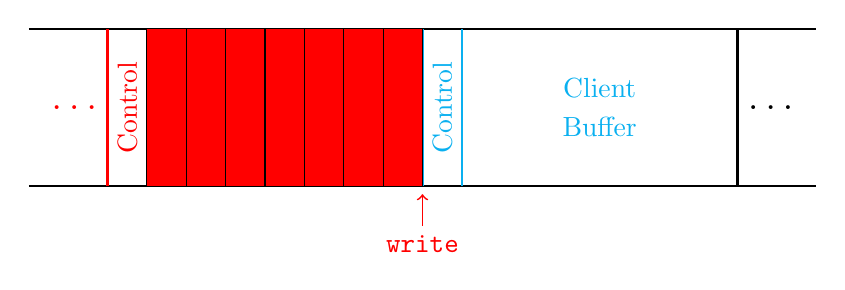
\begin{tikzpicture}

    % Upper/lower border
    \draw [thick] (0, 2) -- ++(10, 0);
    \draw [thick] (0, 0) -- ++(10, 0);

    % Other memory
    \draw [Red, thick] (1, 0) -- ++(0, 2) node [midway, left] {\black\Large $\dots$};
    \draw [thick] (9, 0) -- ++(0, 2)
          node [midway, right] {\black\Large $\dots$};

    % Buffer
    % Control data
    \draw [Red, thick] (1.5, 0) -- ++(0, 2);
    \draw (1.25, 1) node [Red, rotate=90] {Control};

    \draw [ProcessBlue, thick] (5, 0) -- ++(0, 2);
    \draw [ProcessBlue, thick] (5.5, 0) -- ++(0, 2);
    \draw (5.25, 1) node [ProcessBlue, rotate=90] {Control};

    % Server Buffer Label
    \onslide<1>{
      \draw [Red] (3.25, 1.25) node {Server};
      \draw [Red] (3.25, 0.75) node {Buffer};
    }

    \onslide<2->{
      % Server Buffer Memory
      \foreach \i in {0.5, 1, ..., 3} {
        \draw [Red] ({1.5 + \i}, 0) -- ++(0, 2);
      }
    }

    % Labels
    \draw [ProcessBlue] (7.25, 1.25) node {Client};
    \draw [ProcessBlue] (7.25, 0.75) node {Buffer};

    \onslide<3->{
      \foreach \i in {0.5, 1, ..., 3.5} {
        \draw [fill=Red] ({1 + \i}, 0) rectangle ++(0.5, 2);
      }
      \draw [->, semithick, Red]
            (5, -0.5) node [below] {\texttt{write}}
       -- ++(0, 0.4);
    }
  \end{tikzpicture}
\end{slide}

\begin{frame}[fragile]{Implementation}
  \centering
  (4) Server \texttt{write(1.2 MB)}
  \vspace{0.8cm}

  \begin{lstlisting}
    start = now();
    while(not enough space) {
      switch(now() - start) {
        case elapsed_time < LEVEL_ONE: asm("pause");
        case elapsed_time < LEVEL_TWO: sched_yield();
        case elapsed_time < TIMEOUT: usleep(1);
        default: return TIMEOUT_ERROR;
      }
    }
  \end{lstlisting}
\end{frame}

\begin{slide}{Implementation}
  (5) Client \texttt{read(200 KB)}
  \vspace{0.8cm}

  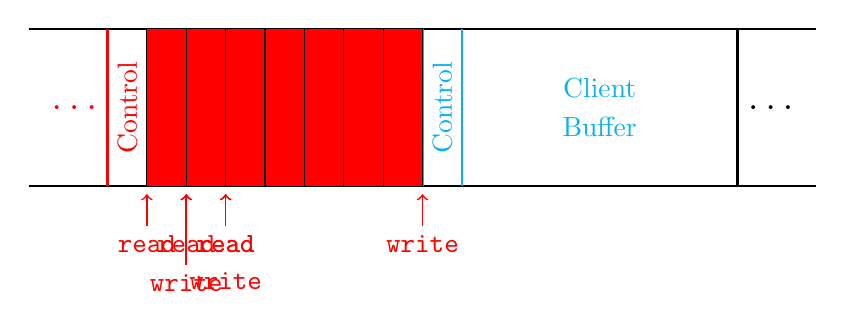
\begin{tikzpicture}

    % Upper/lower border
    \draw [thick] (0, 2) -- ++(10, 0);
    \draw [thick] (0, 0) -- ++(10, 0);

    % Other memory
    \draw [Red, thick] (1, 0) -- ++(0, 2) node [midway, left] {\black\Large $\dots$};
    \draw [thick] (9, 0) -- ++(0, 2)
          node [midway, right] {\black\Large $\dots$};

    % Buffer
    % Control data
    \draw [Red, thick] (1.5, 0) -- ++(0, 2);
    \draw (1.25, 1) node [Red, rotate=90] {Control};

    \draw [ProcessBlue, thick] (5, 0) -- ++(0, 2);
    \draw [ProcessBlue, thick] (5.5, 0) -- ++(0, 2);
    \draw (5.25, 1) node [ProcessBlue, rotate=90] {Control};

    % Server Buffer Memory
    \foreach \i in {0.5, 1, ..., 3} {
      \draw [Red] ({1.5 + \i}, 0) -- ++(0, 2);
    }

    % Labels
    \draw [ProcessBlue] (7.25, 1.25) node {Client};
    \draw [ProcessBlue] (7.25, 0.75) node {Buffer};

    \onslide<-3>{
      \draw [->, semithick, Red]
            (5, -0.5) node [below] {\texttt{write}}
       -- ++(0, 0.4);
    }

    \foreach \i in {1, ..., 7} {
      \ifnum\i<3
        \onslide<-\i>{
          \draw [fill=Red]
                ({1.5+(\i-1)/2}, 0) rectangle ++(0.5, 2);
        }
      \else
       \draw [fill=Red]
             ({1.5+(\i-1)/2}, 0) rectangle ++(0.5, 2);
      \fi
      \ifnum\i<4
       \onslide<\i>{
         \draw [->, semithick, Red]
               ({1.5+(\i-1)/2}, -0.5) node [below] {\texttt{read}}
          -- ++(0, 0.4);
       }
      \fi
    }

    \onslide<4->{
      \draw [->, semithick, Red]
            (2.5, -0.5) node [below] {\texttt{read}}
       -- ++(0, 0.4);
    }

    \foreach \i in {4, 5} {
      \onslide<\i->{
        \draw [fill=Red]
              ({1.5+(\i-4)/2}, 0) rectangle ++(0.5, 2);
      }
    }

    \onslide<4>{
      \draw [->, semithick, Red]
            (2, -1) node [below] {\texttt{write}}
       -- ++(0, 0.9);
    }

    \onslide<5>{
      \draw [Red] (2.5, -1.2) node {\texttt{write}};
    }

  \end{tikzpicture}
\end{slide}

% client write 10 mb
% server read 5 mb
% server write 120 mb
% block
% client read 50 mb
% server write 70 mb
